% Phase 2 IEEE conference source scaffold. The assessed prose must be written
% by Fazal Zaman Khan in his own words. Do not submit this incomplete source.
\documentclass[conference]{IEEEtran}
\usepackage{graphicx}
\usepackage{booktabs}
\usepackage{url}
\usepackage[T1]{fontenc}
\title{FaultPilot: [Author to finalize paper title]}
\author{\IEEEauthorblockN{Fazal Zaman Khan}
\IEEEauthorblockA{Project G2-08, Roll No. 22I-2362\\
Email: fazalzamankhn@gmail.com}}
\begin{document}
\maketitle
\begin{abstract}
% Author: write 150--250 original words with the final measured results.
\end{abstract}
\begin{IEEEkeywords}
automated program repair, agentic AI, debugging, Python
\end{IEEEkeywords}

\section{Introduction}
% Author: motivation, three fixed gaps, research questions and contributions.
\section{Related Work}
% Author: synthesize the verified papers in references.bib and cite each used work.
\section{Problem Formulation}
% Author: define input, output, hypotheses and success criteria.
\section{Proposed System and Methodology}
% Author: explain roles, state, tools and each switchable gap component.
\begin{figure}[t]
\centering
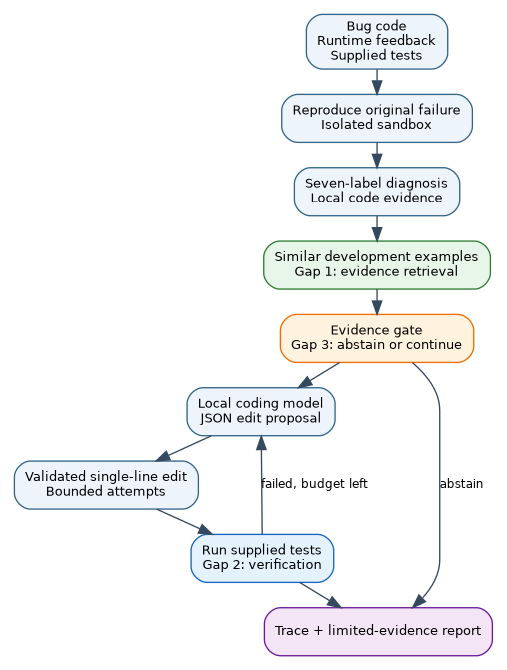
\includegraphics[width=\columnwidth]{architecture.png}
\caption{FaultPilot's implemented bounded repair pipeline and its three gap-specific switches.}
\label{fig:architecture}
\end{figure}
\section{Experimental Setup}
% Author: state split, model digest, decoding, environment, dependencies and budgets.
\section{Evaluation Methodology}
% Author: metric equations, paired comparison, coverage and base-paper boundary.
\section{Results}
% Author: only use numbers generated from the frozen result files.
\InputIfFileExists{tables.tex}{}{}
\section{Ablation and Comparative Analysis}
% Author: report the three switch-off conditions and E6 trade-offs.
\section{Failure Analysis}
% Author: categorize all failures, give frequencies and 2 success/2 failure traces.
\section{Limitations and Threats to Validity}
% Author: address missing dependencies, test oracle limits, small local model,
% and RepairAgent Java-to-Python adaptation.
\section{Conclusion}
% Author: state measured findings and future work without overclaiming.
\bibliographystyle{IEEEtran}
\bibliography{references}
\end{document}
